
El detector CMS, representado de manera esquem\'atica en la Figura~\ref{fig:CMS}, se localiza en uno de los puntos del acelerador LHC donde se hacen colisionar los haces de protones. Est\'a compuesto, de la zona m\'as interna a la m\'as externa, por un tracker de p\'ixeles y tiras de silicio para la detecci\'n de partículas cargadas con gran resoluci\'on espacial, un calor\'metro electromagn\'etico de cristal de tungstato (ECAL) para la medida de electrones y fotones principalmente, un calor\'imetro hadr\'onico constituido de material denso y absorbente (HCAL) especializado en la medida de hadrones, y finalmente, en la parte m\'as externa se encuentran las c\'amaras de muones. Entre el HCAL y las c\'amaras de muones se tiene un im\'an superconductor que alcanza un campo magn\'etico de 3.8 T, suficiente para curvar part\'iculas cargadas y permitir una buena resoluci\'on en la medida del momento de las mismas.

\begin{figure}[h]
\centering
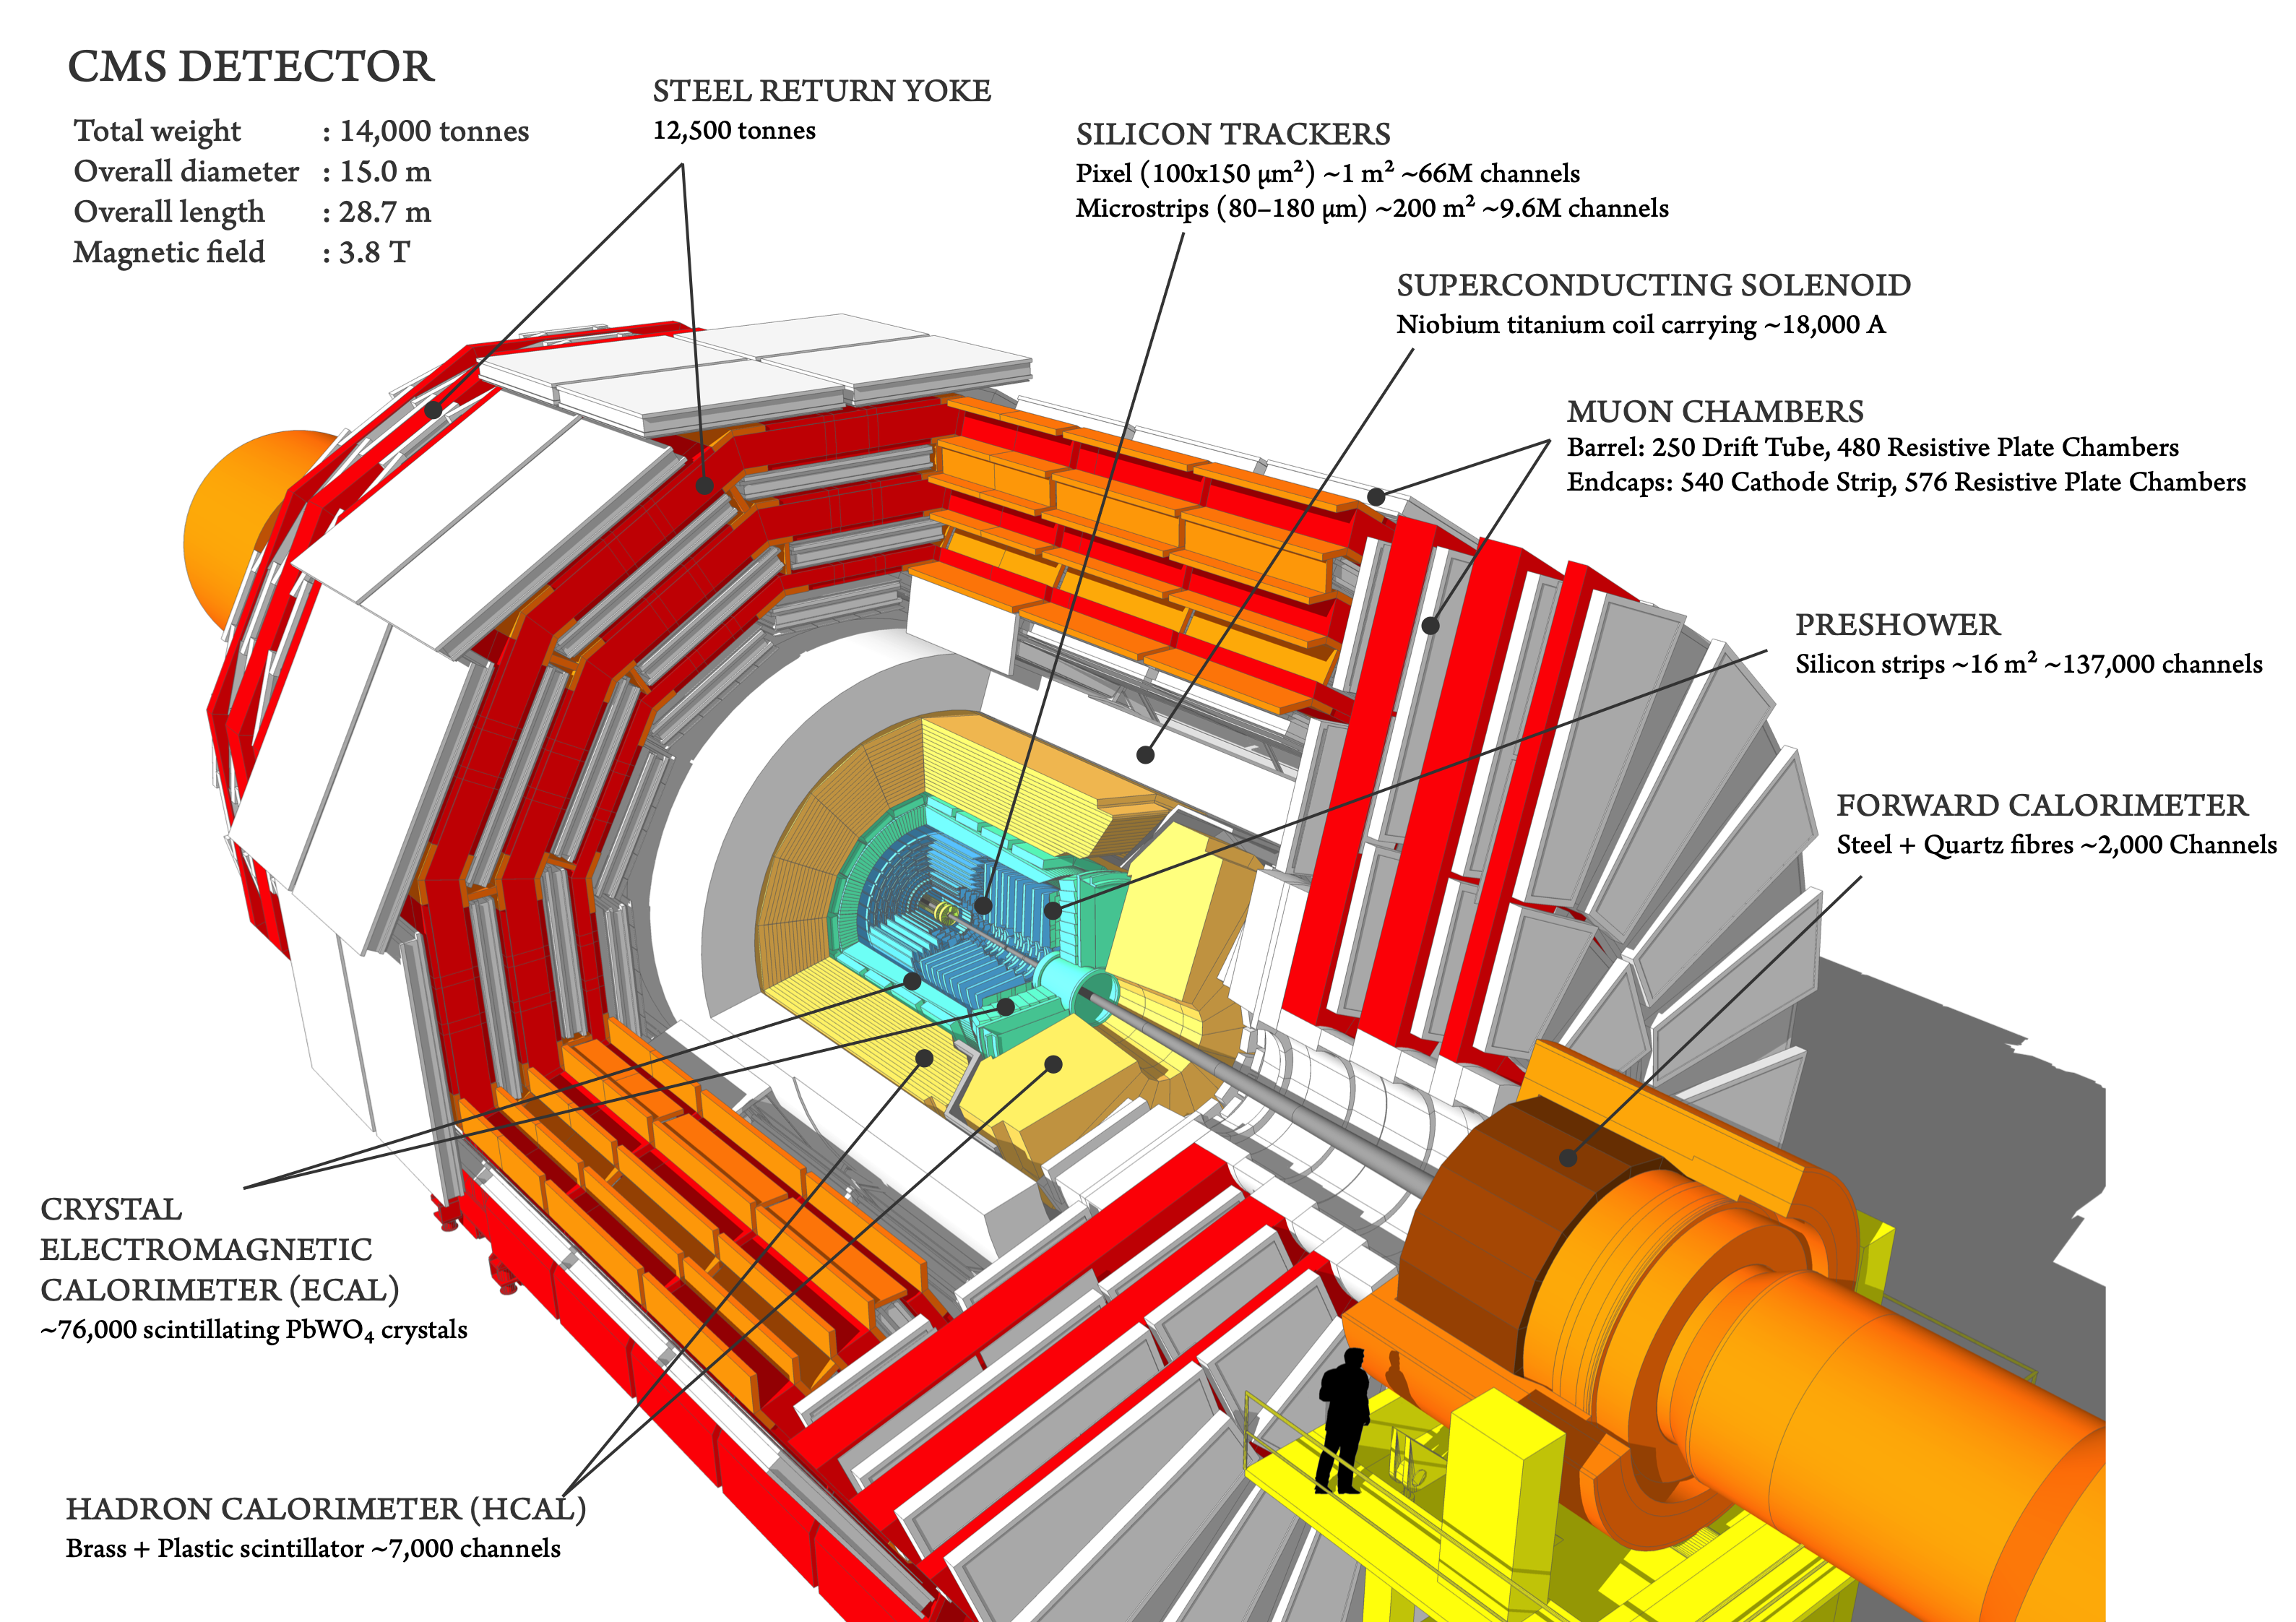
\includegraphics[width=0.80\textwidth]{figures/cms_160312_02.png}
\caption{Representaci\'on gr\'afica de las distintas partes del detector CMS. Imagen tomada de \cite{Sakuma:2665537}.}
\label{fig:CMS}        
\end{figure}

En cuanto a su geometr\'ia, el sistema de coordenadas aceptado tiene como origen el punto de colisi\'on, el eje y apunta verticalmente hacia arriba, el eje x radialmente desde el origen, y el eje z recorre la direcci\'on del haz (ver Figura~\ref{fig:CMS}). El \'angulo azimutal $\phi$ se mide a partir del eje x en el plano x-y transverso al haz, mientras que el \'angulo polar $\theta$ se mide desde el eje z en el plano x-z. Otra variable angular importante que ser\'a utilizada en el an\'alisis por ser invariante bajo transformaciones de Lorentz en el eje z, es la pseudorrapidez $\eta$, que se define en funci\'on del \'angulo polar como: \\

\begin{equation}
  \eta = -\ln\left(\tan\dfrac{\theta}{2}\right)
\label{eq:eta}
\end{equation}


De esta manera, se suelen usar variables definidas en el plano transversal a la dirección del haz de partículas como el momento transverso $p_{T}$ o la energía transversa $E_{T}$. \\

En este trabajo nos centraremos en la medida de los muones, que al ser part\'iculas cargadas dejan se\~nal en el tracker interno, no interaccionan apenas con el material denso de los calor\'imetros, y llegan a las c\'amaras de muones externas, situadas a unos cuatro metros del punto de colisi\'on. \\
En las siguientes subsecciones se describir\'a brevemente el funcionamiento y caracter\'isticas de los detectores de CMS que se utilizan en este trabajo: el tracker, los tubos de deriva o DTs (del ingl\'es \textit{Drift Tubes}), y las c\'amaras de tiras cat\'odicas o CSCs (del ingl\'es \textit{Cathode Strip Chambers}).

\subsection{Tracker}\label{sec:tracker}

El tracker~\cite{trackerperformance} se situa en la parte m\'as interna de CMS y se est\'a formado por p\'ixeles, que se sit\'uan en el n\'ucleo del subdetector y reciben por tanto la mayor intensidad de part\'culas, y por tiras de silicio que rodean las capas de p\'ixeles (ver Figura~\ref{fig:tracker}). \\ 

A medida que las part\'iculas viajan a trav\'es del tracker, los p\'ixeles y las tiras producen peque\~nas se\~nales el\'ectricas que se amplifican y detectan. De esta manera, el tracker cuenta con un total de 75 millones de canales electr\'onicos, dando lugar a unas 6000 conexiones por cent\'imetro cuadrado, consiguiendo medir las trayectorias de las part\'iculas cargadas con una precisi\'on de unos 10 $\mu$m.  \\

\begin{figure}[h]
\centering
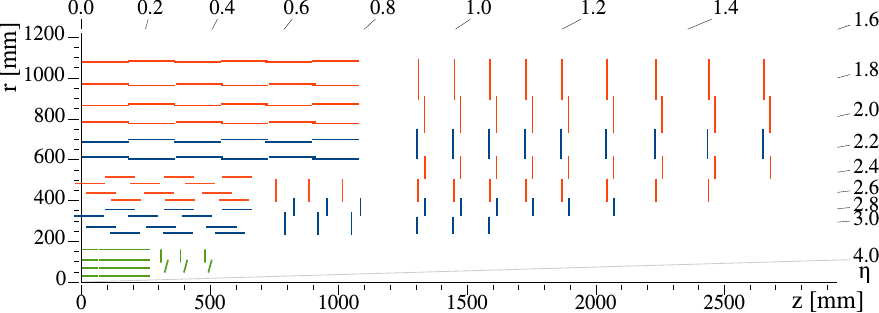
\includegraphics[width=0.9\textwidth]{figures/Phase1_Tracker_1Quarter.png}
\caption{Cuadrante del tracker de CMS en el plano r-z. El detector de p\'ixeles se muestra en verde, mientras que los m\'odulos de tiras de una cara y de dos caras se muestran como segmentos rojos y azules respectivamente. Imagen tomada de \cite{trackerplot}.}
\label{fig:tracker}
\end{figure}


\subsection{Tubos de deriva: DTs}\label{sec:DTs}

Los tubos de deriva~\cite{DTperformance} cubren el barril de CMS ($\lvert \eta \rvert <$ 0.9) en la parte m\'as externa del detector. Cada tubo se compone de un hilo colector de carga cargado positivamente y est\'a lleno de gas, de forma que una part\'icula cargada a su paso por el tubo arranca electrones de los \'atomos del gas, que son atraidos el\'ectricamente y recolectados por el hilo conductor. De esta manera, se obtienen las coordenadas del paso del mu\'on por el tubo a partir de la posici\'on del hilo donde los electrones impactan y de la distancia del mu\'on al hilo, que se calcula multiplicando la velocidad de deriva del electr\'on en el tubo por el tiempo de viaje hasta el hilo. \\

El subdetector completo consta de 250 c\'amaras, cada una de ellas con unas dimensiones en promedio de 2 x 2.5 m, estando formadas por de tres capas con unos 60 tubos repartidos en cuatro subcapas. \\
En la Figura~\ref{fig:CMSsub} se representa gr\'aficamente la posici\'on espacial de las distintas c\'amaras que forman las DTs, que se denotan como MBZ/N/S, donde Z=-2...+2 se corresponde con el n\'umero de rueda a lo largo del eje z, N=1...4 hace referencia al n\'umero de estaci\'on conc\'entrica en el plano xy, y S=1...12 al n\'umero de sector circular. 


\subsection{C\'amaras de tiras cat\'odicas: CSCs}\label{sec:CSCs}

Las c\'amaras de tiras cat\'odicas~\cite{CSCperformance} se localizan en las tapas de CMS (1.2 $< \lvert \eta \rvert <$ 2.4) y su funcionamiento es similar al de las DTs. En este caso se tienen cables de cargados positivamente (\'anodos) cruzados con tiras de de cobre cargadas negativamente (c\'atodos) dentro de un volumen de gas. Cuando los muones atraviesan la c\'amara arrancan electrones de los \'atomos de gas, produci\'endose una avalancha de electrones que se dirigen a los cables del \'anodo, mientras que los iones positivos se alejan del cable y se dirigen al c\'atodo de cobre, lo que tambi\'en induce un pulso de carga en las tiras (en direcci\'on perpendicular al \'anodo). Debido a que las tiras y los cables son perpendiculares, se obtienen dos coordenadas de posici\'on para cada part\'icula que atraviesa la c\'amara. \\

\begin{figure}[h]
\centering
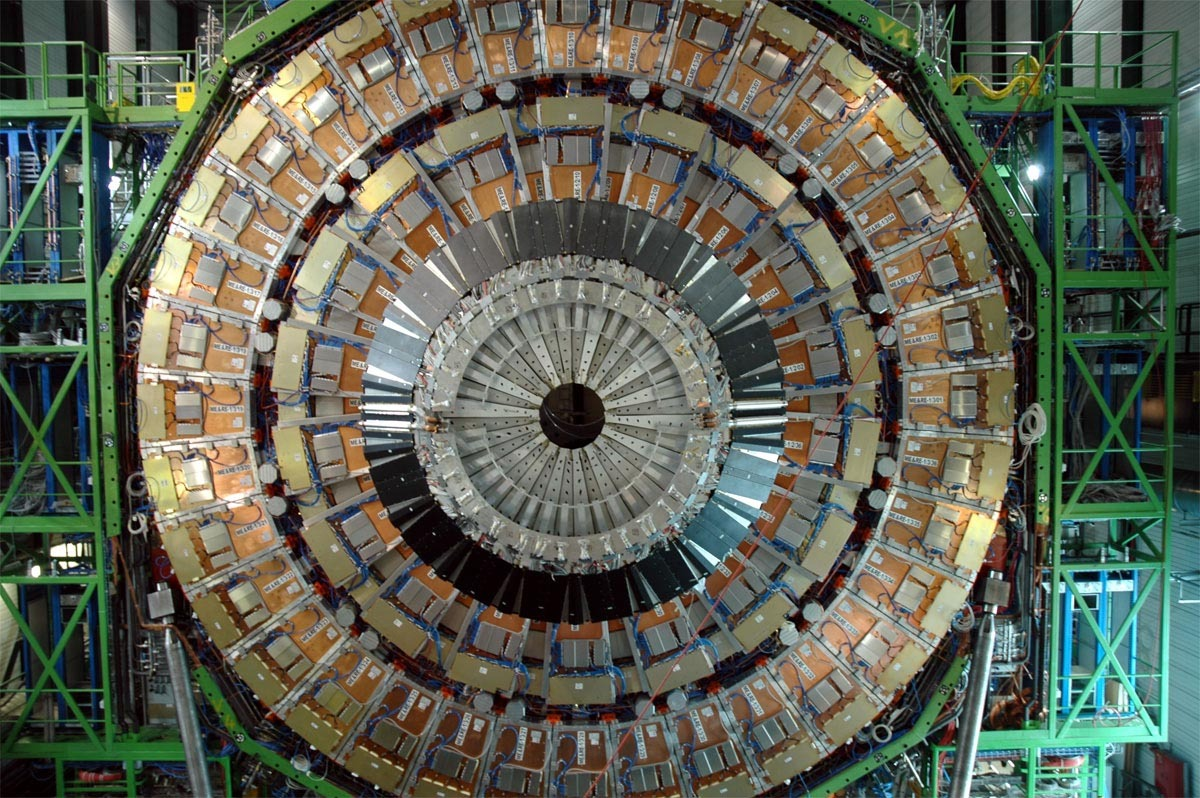
\includegraphics[width=0.60\textwidth]{figures/CSC_MEm1.jpg}
\caption{Foto completa de la estaci\'on ME-1. Imagen tomada de \cite{Breedon:1431505}.}
\label{fig:CSC_MEm1}        
\end{figure}


El subdetector completo de las CSCs contiene 540 c\'amaras en total, y est\'a compuesto de anillos de c\'amaras trapezoidales de hasta 3.4 m de largo y 1.5 m de ancho, colocadas en ocho discos, cuatro en cada tapa. \\
En este caso, las c\'amaras CSCs se denotan espacialmente como ME$\pm$S/R, donde el signo indica en qu\'e tapa de CMS se encuentra, S=1...4 hace referencia al n\'umero de estaci\'on, paralelas en el eje z (ver Figura~\ref{fig:CMSsub}), y R se corresponde con el n\'umero de anillo, conc\'entricos en el plano xy. En la Figura~\ref{fig:CSC_MEm1} se muestra una imagen real de la rueda ME-1, con sus tres anillos conc\'entricos en el plano xy. \\ \\ 

\begin{figure}
\centering
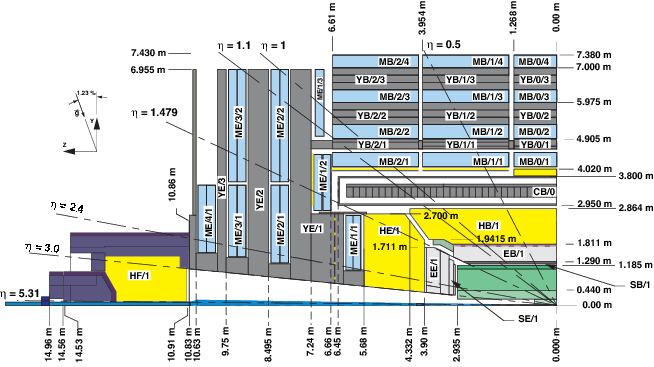
\includegraphics[width=0.8\textwidth]{figures/CMSview1.png}
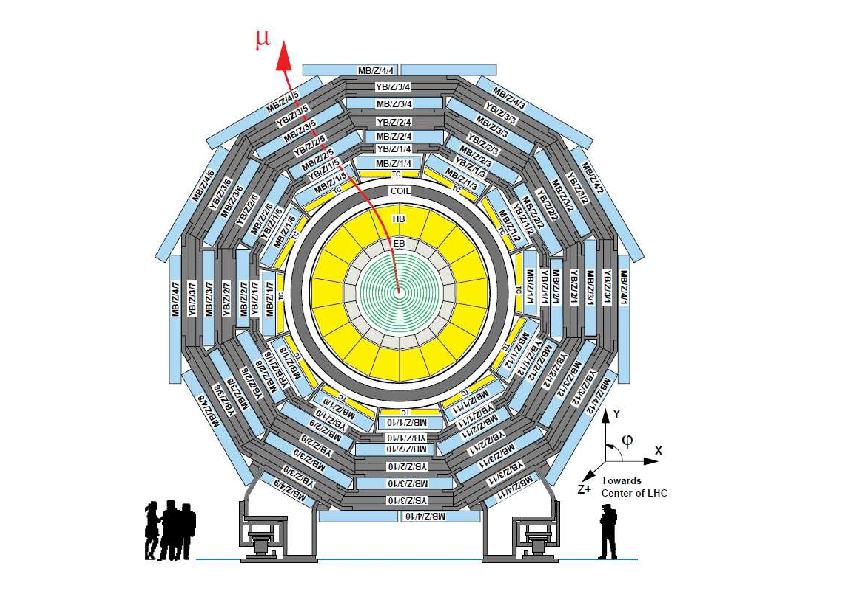
\includegraphics[width=0.8\textwidth]{figures/CMSview.png}
\caption{Vista esquem\'atica del detector CMS. Arriba: vista longitudinal de un cuarto del detector. Abajo: vista transversal en $z = 0$. Ambas figuras han sido tomadas de \cite{DTperformance}.}
\label{fig:CMSsub}
\end{figure}


Cada una de las c\'amaras de DTs y CSCs se compone de varias capas, y las se\~nales o impactos que dejan los muones a su paso se reconstruyen en cada cada de ellas. A partir de estos impactos, se construyen trazas rectas denominadas segmentos uniendo las se\~nales encontradas en las distintas capas dentro de cada c\'amara DT o CSC. De esta manera, como se detallar\'a en las sucesivas secciones, se utilizar\'an en el an\'alisis los segmentos que los muones dejan a su paso por las distintas c\'amaras.

\clearpage
